\chapter{浮動小数点数と固定小数点数についての基礎知識}
\label{chap:基礎知識1}
計算機内部で扱う数値には二つの表現方法がある.
それぞれの表現方法を固定小数点数と浮動小数点数という.
これらの表現方法について説明する.
固定小数点数,浮動小数点数を説明するために,いくつかの記号を導入する.
実数全体の集合,整数全体の集合,自然数全体の集合はそれぞれ$ \R, \Z, \N$と表すのに対して,計算機の中で表現できる数全体の集合を$\mathbb{F} \ (\subset \R)$と表す.
特に,固定小数点全体の集合,浮動小数点全体の集合はそれぞれ$\fixnum,\flonum$と表す.



\section{固定小数点}
固定小数点数は,与えられたbit数に対して,そのうち小数部にいくつのbitを割り当てるのかを決めて残りのbitを整数部に割り当てて数を表現する方法である.
例として,$N \in \N$として計算機の中で$N$bitが数字を記憶するために与えられているとする.
そのうち,$m \ (m < N)$bitを小数部に割り当てた固定小数点数$a = a_{N-m-1} a_{N-m-2} \cdots a_1 a_0. a_{-1} \cdots a_{-m} \ (\in \fixnum)$の値は,符号を考えない場合は以下のようになる:

\begin{align*}
    a =& a_{N-m-1} 2^{N-m-1} + a_{N-m-2} 2^{N-m-2} + \cdots + a_1 2^1 + a_0 2^0 \\
    & + a_{-1} 2^{-1} + \cdots + a_{-m} 2^{-m}.
\end{align*}
ただし,$a_{i} \ (i = N-m-1,N-m-2,\dots,1,0,-1,\dots,-m)$は$0$または$1$の値を取る.
\begin{figure}[H]
    \centering
    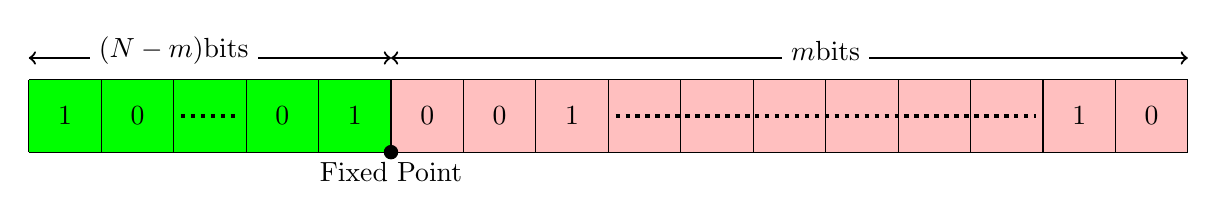
\begin{tikzpicture}[scale=0.92]
        \fill[green] (0,0) rectangle (5,1);
        \fill[pink] (5,0) rectangle (16,1);
        \draw (0,0) grid (16,1);
        \fill (5,0) circle [radius=0.1] node [below] {Fixed Point};
        \draw[ultra thick, dotted] (2.1,0.5) -- (2.9,0.5);
        \node [anchor=center] at (0.5,0.5) {1};
        \node [anchor=center] at (1.5,0.5) {0};
        \node [anchor=center] at (3.5,0.5) {0};
        \node [anchor=center] at (4.5,0.5) {1};
        \node [anchor=center] at (5.5,0.5) {0};
        \node [anchor=center] at (6.5,0.5) {0};
        \node [anchor=center] at (7.5,0.5) {1};
        \draw[ultra thick, dotted] (8.1,0.5) -- (13.9,0.5);
        \node [anchor=center] at (14.5,0.5) {1};
        \node [anchor=center] at (15.5,0.5) {0};
        \draw[<->,thick] (0,1.3) -- (5,1.3);
        \draw (2,1.4) node[fill=white] {$\small (N-m)$bits};
        \draw[<->,thick] (5,1.3) -- (16,1.3);
        \draw (11,1.4) node[fill=white] {$m$bits};
    \end{tikzpicture}
    \caption{$N$bitの符号なし固定小数点のイメージ図.}
    \label{fig:fixedpointnumber_unsigned}
\end{figure}
また,符号付き固定小数点の場合,符号に$1$bit割り当てるため整数部が$N-m-1$bitとなる.
$s$を符号とすると,符号付き固定小数点数$a_{\mathrm{signed}} = s a_{N-m-2} a_{N-m-3} \cdots a_1 a_0. a_{-1} \cdots a_{-m} \ (\in \fixnum)$の値は以下のようになる:
\begin{align*}
    a_{\mathrm{signed}} =& (-1)^s \left( a_{N-m-2} \times 2^{N-m-2} + a_{N-m-3} \times 2^{N-m-3} + \cdots \right. \\
     &\left. + a_{1} \times + 2^{1} + a_{0} \times 2^{0}+ a_{-1} \times 2^{-1} +  \cdots + a_{-m} \times 2^{-m} \right).
\end{align*}
\begin{figure}[H]
    \centering
    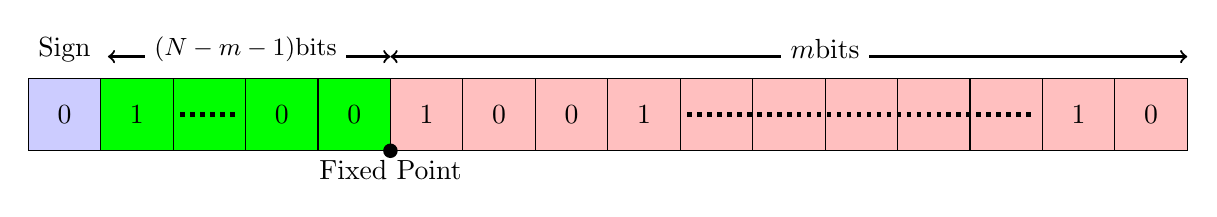
\begin{tikzpicture}[scale=0.92]
        \fill[green] (1,0) rectangle (5,1);
        \fill[pink] (5,0) rectangle (16,1);
        \fill[blue, opacity=0.2] (0,0) rectangle (1,1);
        \draw (0,0) grid (16,1);
        \fill (5,0) circle [radius=0.1] node [below] {Fixed Point};
        \draw[ultra thick, dotted] (2.1,0.5) -- (2.9,0.5);
        \node [anchor=center] at (0.5,0.5) {0};
        \node [anchor=center] at (1.5,0.5) {1};
        \node [anchor=center] at (3.5,0.5) {0};
        \node [anchor=center] at (4.5,0.5) {0};
        \node [anchor=center] at (5.5,0.5) {1};
        \node [anchor=center] at (6.5,0.5) {0};
        \node [anchor=center] at (7.5,0.5) {0};
        \node [anchor=center] at (8.5,0.5) {1};
        \draw[ultra thick, dotted] (9.1,0.5) -- (13.9,0.5);
        \node [anchor=center] at (14.5,0.5) {1};
        \node [anchor=center] at (15.5,0.5) {0};
        \draw[<->,thick] (1.1,1.3) -- (5,1.3);
        \draw[<->,thick] (5,1.3) -- (16,1.3);
        \draw (3,1.4) node[fill=white,font=\small] {$(N-m-1)$bits};
        \draw (11,1.4) node[fill=white] {$m$bits};
        \draw (0.5,1.4) node[fill=white] {Sign};
    \end{tikzpicture}
    \caption{$N$bitの符号付き固定小数点のイメージ図.}
    \label{fig:fixedpointnumber_signed}
\end{figure}
本論文では,$N$bitの符号付き固定小数点で小数部に$m$bit,整数部に$(N-m-1)$bitを割り当てた固定小数点を,
\begin{equation}
    \text{Q}(N-m-1)\text{f}m
\end{equation}
と表す.
例えば,Q11f52は符号に1bit,小数部に52bit,整数部に11bitを割り当てた固定小数点数のことを表す.
また,以降は小数部を固定した特定の固定小数点全体の集合を$\fixnumcustom{11}{52}$などと表すこととする.
\section{浮動小数点}
浮動小数点は,与えられたbit数に対して,bitを仮数部と指数部にわけて数を表現する方法である.
仮数部の数を$m \ (\in \Z)$,指数部の数を$e \ (\in \Z)$とすると浮動小数点$b \ (\in \flonum)$は,以下の様に表現できる:
\begin{align*}
    b = m \times 2^e.
\end{align*}
ここで$m,e$はともに2進数の数である.
浮動小数点については,国際的な規格があり,割り当てられるbit数が32bit,64bitのものをそれぞれ単精度浮動小数点(Float32),倍精度浮動小数点(Float64)という.
それぞれの浮動小数点数の仮数部と指数部のbit数は以下の表のように決められている:
\begin{table}[H]
    \centering
    \caption{単精度浮動小数点(Float32)と倍精度浮動小数点(Float64)の仮数部と指数部のbit数.}
    \begin{tabular}{c|c|c}   
     & 仮数部 & 指数部 \\ \hline
    Float32 & 23bit & 8bit \\ 
    Float64 & 52bit & 11bit
    \end{tabular}
    \label{tab:Float32_Float64_bit}
\end{table}
以降,単精度浮動小数点全体の集合,倍精度浮動小数点全体の集合を$\floatsigle,\floatdouble$などと表すこととする.
単精度浮動小数点(Float32)の割り当ては以下の様になる:
\begin{figure}[H]
    \centering
    \begin{tikzpicture}[scale=0.92]
        \fill[green] (1,0) rectangle (5,1);
        \fill[pink] (5,0) rectangle (16,1);
        \fill[blue, opacity=0.2] (0,0) rectangle (1,1);
        \draw (0,0) grid (16,1);
        \draw[ultra thick, dotted] (2.1,0.5) -- (2.9,0.5);
        \node [anchor=center] at (0.5,0.5) {0};
        \node [anchor=center] at (1.5,0.5) {1};
        \node [anchor=center] at (3.5,0.5) {0};
        \node [anchor=center] at (4.5,0.5) {0};
        \node [anchor=center] at (5.5,0.5) {1};
        \node [anchor=center] at (6.5,0.5) {0};
        \node [anchor=center] at (7.5,0.5) {0};
        \node [anchor=center] at (8.5,0.5) {1};
        \draw[ultra thick, dotted] (9.1,0.5) -- (13.9,0.5);
        \node [anchor=center] at (14.5,0.5) {1};
        \node [anchor=center] at (15.5,0.5) {0};
        \draw[<->,thick] (1.1,1.3) -- (5,1.3);
        \draw[<->,thick] (5,1.3) -- (16,1.3);
        \draw (3,1.4) node[fill=white] {指数部$8$bits};
        \draw (11,1.4) node[fill=white] {仮数部$23$bits};
        \draw (0.5,1.4) node[fill=white] {Sign};
    \end{tikzpicture}
    \caption{単精度浮動小数点(Float32)のイメージ図.}
    \label{fig:float32_bit}
\end{figure}
単精度浮動小数点(Float32)は,指数部の8bitで整数値では$0 \sim  255$の値を取るが$-127$のバイアスがある.
つまり,実際の指数部の数は計算機内で表せる2進数の数から$127$を引いた数となっている.
また,仮数部の値は暗黙に一つ上の位が$1$であるとして,小数点以下の位を表す表現方法を用いている.
よって,単精度浮動小数点で表せられる値$b_{32} \ (\in \floatsigle)$は,指数部の数を$e_{32}$,仮数部の各bitを$b_{-1}$,$b_{-2}$,...,$b{-23}$とすると,
\begin{align*}
    b_{32} &= (-1)^{\mathrm{sign}}(1 + b_{-1}\times 2^{-1} + b_{-2}\times 2^{-2} + \cdots + b_{-23}\times 2^{-23})\times 2^{e_{32} - 127} \\
        &= (-1)^{\mathrm{sign}}\left(1 + \sum_{i = 1}^{23} b_{-i} 2^{-i}\right)\times 2^{e_{32} - 127}
\end{align*}
となる.
倍精度浮動小数点(Float64)の割り当ては以下の様になる:
\begin{figure}[H]
    \centering
    \begin{tikzpicture}[scale=0.92]
        \fill[green] (1,0) rectangle (5,1);
        \fill[pink] (5,0) rectangle (16,1);
        \fill[blue, opacity=0.2] (0,0) rectangle (1,1);
        \draw (0,0) grid (16,1);
        \draw[ultra thick, dotted] (2.1,0.5) -- (2.9,0.5);
        \node [anchor=center] at (0.5,0.5) {0};
        \node [anchor=center] at (1.5,0.5) {1};
        \node [anchor=center] at (3.5,0.5) {0};
        \node [anchor=center] at (4.5,0.5) {0};
        \node [anchor=center] at (5.5,0.5) {1};
        \node [anchor=center] at (6.5,0.5) {0};
        \node [anchor=center] at (7.5,0.5) {0};
        \node [anchor=center] at (8.5,0.5) {1};
        \draw[ultra thick, dotted] (9.1,0.5) -- (13.9,0.5);
        \node [anchor=center] at (14.5,0.5) {1};
        \node [anchor=center] at (15.5,0.5) {0};
        \draw[<->,thick] (1.1,1.3) -- (5,1.3);
        \draw[<->,thick] (5,1.3) -- (16,1.3);
        \draw (3,1.4) node[fill=white] {指数部$11$bits};
        \draw (11,1.4) node[fill=white] {仮数部$52$bits};
        \draw (0.5,1.4) node[fill=white] {Sign};
    \end{tikzpicture}
    \caption{倍精度浮動小数点(Float64)のイメージ図.}
    \label{fig:float64_bit}
\end{figure}
倍精度浮動小数点(Float64)は指数部の11bitで整数値では$0 \sim  2047$の値を取るが$-1023$のバイアスがある.
また,単精度浮動小数点と同様に仮数部の値は暗黙に一つ上の位が$1$であるとして,小数点以下の位を表す表現方法を用いている.
よって,倍精度浮動小数点で表せられる値$b_{64} \ (\in \floatdouble)$は,指数部の数を$e_{64}$,仮数部の各bitを$b_{-1}$,$b_{-2}$,...,$b{-52}$とすると,
\begin{align*}
    b_{64} &= (-1)^{\mathrm{sign}}(1 + b_{-1}\times 2^{-1} + b_{-2}\times 2^{-2} + \cdots + b_{-52}\times 2^{-52})\times 2^{e_{64} - 1023} \\
        &= (-1)^{\mathrm{sign}}\left(1 + \sum_{i = 1}^{52} b_{-i} 2^{-i}\right)\times 2^{e_{64} - 1023}
\end{align*}
となる.
以上から浮動小数点はbit数によって表現出来る数の範囲が異なる.
単精度浮動小数点と倍精度浮動小数点では以下の様になる:
\begin{table}[H]
    \centering
        \caption{単精度浮動小数点と倍精度浮動小数点の表現可能な数の範囲.}
        \small
        \begin{tabular}{p{3em}|>{\centering}p{11em}|>{\centering}p{11em}|c}   
            & 最大値 & 最小 & 0に最も近い数 \\ \hline \hline
            {\scriptsize Float32} &
            \begin{tabular}{c}
                ${\scriptsize\sum_{i=105}^{128}2^i}$ \\
                ${\scriptsize\backsimeq 3.402824\times 10^{38}}$
            \end{tabular}&
            \begin{tabular}{c}
                ${\scriptsize-\sum_{i=105}^{128}2^i}$ \\
                ${\scriptsize\backsimeq -3.402824\times 10^{38}}$
            \end{tabular}&
            \begin{tabular}{c}
                ${\scriptsize2^{-127}}$ \\
                ${\scriptsize\backsimeq 1.175494\times 10^{-38}}$
            \end{tabular} \\ \hline
            {\scriptsize Float64} &
            \begin{tabular}{c}
                ${\scriptsize\sum_{i=927}^{1024}2^i}$ \\
                ${\scriptsize\backsimeq 1.797693\times 10^{308}}$
            \end{tabular}&
            \begin{tabular}{c}
                ${\scriptsize-\sum_{i=927}^{1024}2^i}$ \\
                ${\scriptsize\backsimeq -1.797693\times 10^{308}}$
            \end{tabular}&
            \begin{tabular}{c}
                ${\scriptsize2^{-1023}}$ \\
                ${\scriptsize\backsimeq 2.225074\times 10^{-308}}$
            \end{tabular}
        \end{tabular}
        \label{tab:Float32_Float64_range}
\end{table}

以上のように,固定小数点数と浮動小数点数には表現出来る数の値に違いある.
そのイメージを表したのが以下の図である.
\begin{figure}[H]
    \centering
    \begin{tikzpicture}
        \draw [->, thick] (-7,0) -- (7,0);
        \draw [thick] (-6,0.2) -- (-6,-0.2);
        \draw [thick] (-5,0.2) -- (-5,-0.2);
        \draw [thick] (-4,0.2) -- (-4,-0.2);
        \draw [thick] (-3,0.2) -- (-3,-0.2);
        \draw [thick] (-2,0.2) -- (-2,-0.2);
        \draw [thick] (-1,0.2) -- (-1,-0.2);
        \draw [thick] (0,0.5) -- (0,-0.5) node [below] {0};
        \draw [thick] (1,0.2) -- (1,-0.2);
        \draw [thick] (2,0.2) -- (2,-0.2);
        \draw [thick] (3,0.2) -- (3,-0.2);
        \draw [thick] (4,0.2) -- (4,-0.2);
        \draw [thick] (5,0.2) -- (5,-0.2);
        \draw [thick] (6,0.2) -- (6,-0.2);
    \end{tikzpicture}
    \caption{固定小数点数の値として表せる数のイメージ図,横線が数直線,縦線が表現出来る数を示す.}
    \label{fig:fixedpoint_image}
\end{figure}

\begin{figure}[H]
    \centering
    \begin{tikzpicture}
        \draw [->, thick] (-7,0) -- (7,0);
        \draw [thick] (-4,0.2) -- (-4,-0.2);
        \draw [thick] (-2,0.2) -- (-2,-0.2);
        \draw [thick] (-1,0.2) -- (-1,-0.2);
        \draw [thick] (-0.5,0.2) -- (-0.5,-0.2);
        \draw [thick] (-0.25,0.2) -- (-0.25,-0.2);
        \draw [thick] (-0.125,0.2) -- (-0.125,-0.2);
        \draw [thick] (0,0.5) -- (0,-0.5) node [below] {0};
        \draw [thick] (0.125,0.2) -- (0.125,-0.2);
        \draw [thick] (0.25,0.2) -- (0.25,-0.2);
        \draw [thick] (0.5,0.2) -- (0.5,-0.2);
        \draw [thick] (1,0.2) -- (1,-0.2);
        \draw [thick] (2,0.2) -- (2,-0.2);
        \draw [thick] (4,0.2) -- (4,-0.2);
    \end{tikzpicture}
    \caption{浮動小数点数の値として表せる数のイメージ図,横線が数直線,縦線が表現出来る数を示す.}
    \label{fig:floatpoint_image}
\end{figure}
図(\ref{fig:fixedpoint_image})のように固定小数点数で表せる数で隣り合う数は隣の数までの間隔が一定である.
それに対して図(\ref{fig:floatpoint_image})のように浮動小数点数で表せる数で隣り合う数は隣の数までの間隔が一定ではない.
浮動小数点数で表せる数で2つの隣り合う数は,$0$に近い値ほど間隔が小さく密になり,$0$から離れるほど指数的に大きくなる.


図(\ref{fig:fixedpoint_image}),(\ref{fig:floatpoint_image})で表したように,固定小数点,浮動小数点ともに計算機の中で表すことのできる数は限られている.